\documentclass[aspectratio=169]{beamer}

\usetheme{Madrid}
\usecolortheme{default}

% SCR Colors
\definecolor{scrdarkblue}{RGB}{30,90,160}
\definecolor{scrblue}{RGB}{60,140,230}
\definecolor{scrlightblue}{RGB}{235,245,255}
\definecolor{accentorange}{RGB}{255,140,50}

% Apply colors to theme
\setbeamercolor{palette primary}{bg=scrdarkblue,fg=white}
\setbeamercolor{palette secondary}{bg=scrblue,fg=white}
\setbeamercolor{palette tertiary}{bg=scrdarkblue,fg=white}
\setbeamercolor{palette quaternary}{bg=scrblue,fg=white}
\setbeamercolor{structure}{fg=scrdarkblue}
\setbeamercolor{section in toc}{fg=scrdarkblue}
\setbeamercolor{subsection in head/foot}{bg=scrlightblue,fg=scrdarkblue}

% Softer alert blocks (avoid heavy red banners)
\setbeamercolor{alertblock title}{bg=scrblue,fg=white}
\setbeamercolor{alertblock body}{bg=scrlightblue,fg=black}

% Remove navigation symbols
\setbeamertemplate{navigation symbols}{}


% Footer (lighter + less dominant)
\setbeamercolor{author in head/foot}{bg=scrlightblue,fg=scrdarkblue}
\setbeamercolor{title in head/foot}{bg=scrlightblue,fg=scrdarkblue}
\setbeamercolor{date in head/foot}{bg=scrlightblue,fg=scrdarkblue}
\setbeamerfont{author in head/foot}{size=\scriptsize}
\setbeamerfont{title in head/foot}{size=\scriptsize}
\setbeamerfont{date in head/foot}{size=\scriptsize}

\setbeamertemplate{footline}{
  \leavevmode%
  \hbox{%
    \begin{beamercolorbox}[wd=.34\paperwidth,ht=2.0ex,dp=0.9ex,left]{author in head/foot}%
      \hspace*{1.2ex}\insertshortauthor
    \end{beamercolorbox}%
    \begin{beamercolorbox}[wd=.44\paperwidth,ht=2.0ex,dp=0.9ex,center]{title in head/foot}%
      \insertshorttitle
    \end{beamercolorbox}%
    \begin{beamercolorbox}[wd=.22\paperwidth,ht=2.0ex,dp=0.9ex,right]{date in head/foot}%
      \insertshortdate{}\hspace*{1.2ex}\insertframenumber{} / \inserttotalframenumber\hspace*{1.2ex}
    \end{beamercolorbox}%
  }%
  \vskip0pt%
}


% Packages
\usepackage{graphicx}
\usepackage{booktabs}
\usepackage{listings}
\usepackage{tikz}
\usepackage{hyperref}
\usepackage{tikz}
\usetikzlibrary{positioning}



% Background watermark (used only on selected slides)
\newcommand{\watermark}{
    \usebackgroundtemplate{
        \tikz[remember picture,overlay] 
        \node[opacity=0.4] at (current page.east)
        {\includegraphics[width=0.8\paperwidth]{../images/surrey-stag.png}
        };
    }
}



% Title page info
\title{Under the Hood:}
\subtitle{A Deep Dive into Portfolio Optimisation}
\author{SCR Quantitative Research Division}
\institute{Surrey Capital Research, University of Surrey}
\date{February 2026}
\begin{document}

% Title slide
{
\watermark
\begin{frame}
\titlepage

\end{frame}
}
% The Research Objective
\begin{frame}{The Research Objective}
\begin{center}
\Large
\begin{block}{Primary Question}
Do sophisticated portfolio optimisation models outperform basic models in out-of-sample testing?
\end{block}

\vspace{1cm}

\normalsize
\textcolor{scrblue}{\textbf{If you have £100,000 to invest across stocks, bonds, precious metals and commodities. \\ How should it be allocated?}}

\vspace{1cm}
\textbf{We're testing this empirically.}
\end{center}
\end{frame}

% Motivation
\begin{frame}{Motivation}

\Large
Portfolio optimisation is central to modern finance, investors rely on mathematical models to allocate capital.

\vspace{0.4cm}

\normalsize
However:

\begin{itemize}
\item Empirical evidence suggests naive strategies often perform competitively.
\item Market conditions shift across regimes.
\item Increased model complexity may not always translate into better outcomes.
\end{itemize}

\vspace{0.4cm}

\small
\centering
\textit{This is a live debate in quantitative finance — theory vs. practice.}
\end{frame}

% Investment Universe
\begin{frame}{Our Investment Universe}
\begin{table}
\centering
\begin{tabular}{l l r}
\toprule
\textbf{Asset Class} & \textbf{Examples} & \textbf{Count} \\
\midrule
UK Equities & HSBC, BP, Shell, Tesco, etc... & 15 \\
UK Government Bonds & iShares Core UK Gilts ETF & 1 \\
Precious Metals & Invesco Physical Gold ETC & 1 \\
Commodities & WisdomTree Commodities ETF & 1 \\
\midrule
\textbf{Total} & \textbf{Multi-Asset Portfolio} & \textbf{18} \\
\bottomrule
\end{tabular}
\end{table}

\vspace{0.5cm}

\textbf{Data period:} 2015–2025 (10 years)
\begin{itemize}
    \item Including major stress regimes
    \item Daily prices
    \item Monthly rebalancing
\end{itemize}
\end{frame}

% The Models - Overview
\begin{frame}{The Four Strategies We're Testing}
\begin{enumerate}
    \item \textbf{Equal Weight (1/N)} — Naive baseline
    \vspace{0.3em}
    \item \textbf{Mean-Variance Optimisation (MVO)} — Markowitz (1952)
    \vspace{0.3em}
    \item \textbf{Black-Litterman} — Bayesian equilibrium + views
    \vspace{0.3em}
    \item \textbf{Risk Parity} — Equal risk contribution
\end{enumerate}

\vspace{1em}
\begin{center}
\textcolor{scrblue}{\textbf{All tested on identical data with identical methodology}}
\end{center}
\end{frame}

% Model 1: Equal Weight
\begin{frame}{Strategy 1: Equal Weight }
\begin{block}{The Benchmark}
Simplest possible: split money equally across all 18 assets
\end{block}


\begin{center}
\Large
\[ w_i = \frac{1}N{}\]
\end{center}
\vspace{1cm}

\normalsize

DeMiguel et al (2009): Equal weight often beats sophisticated models due to estimation error in expected returns and covariances.


\end{frame}

% Model 2: MVO
\begin{frame}{Strategy 2: Mean-Variance Optimisation}
\begin{block}{Markowitz (1952) — Foundation of Modern Portfolio Theory}
Maximize return for given risk (or minimize risk for given return)
\end{block}

\vspace{0.5em}

\Large
\[
\max_{w} \frac{w^T \mu - r_f}{\sqrt{w^T \Sigma w}} \quad \text{s.t.} \quad \sum w_i = 1, \, w_i \geq 0
\]

\vspace{1cm}
\normalsize
Highly sensitive to $\mu$ and $\Sigma$ estimation and can produce extreme, unstable allocations out-of-sample.

\end{frame}

% Model 3: Black-Litterman
\begin{frame}{Strategy 3: Black-Litterman Model}
\begin{block}{ Fischer Black and Robert Litterman (1992) - Global Portfolio Optimisation }
    Model was created as an enhancement to MVO which overcomes instability by anchoring to market equilibrium.
\end{block}
\vspace{0.5cm}

\begin{center}
\Large
Posterior Returns = Equilibrium + Investor Views
\end{center}

\vspace{0.5cm}

\normalsize
\begin{itemize}
    \item Posterior Returns $\rightarrow$ A complex, weighted average which generates an estimate of expected returns.
    \item Equilibrium $\rightarrow$ A neutral, market capitalisation-weighted returns
    \item Investor Views $\rightarrow$ A non-neutral view on asset returns which is weighted by confidence.
\end{itemize}

\vspace{0.5cm}


\end{frame}

% Model 4: Risk Parity
\begin{frame}{Strategy 4: Risk Parity}
\begin{block}{Equal Risk Contribution, Not Equal Capital}
The philosophy of this model is to diversify risk with a structural bias to low-volatility assets.
\end{block}

\vspace{0.5cm}

\Large
\[
w_i \times \frac{\partial \sigma_p}{\partial w_i} = \frac{\sigma_p}{N}
\]

\vspace{0.5cm}
\normalsize
Allocates capital to equalise marginal risk contribution ensuring no single asset or sector is dominant in the portfolio.

\end{frame}

% Backtesting Methodology
\begin{frame}{Backtesting Engine}
\begin{center}
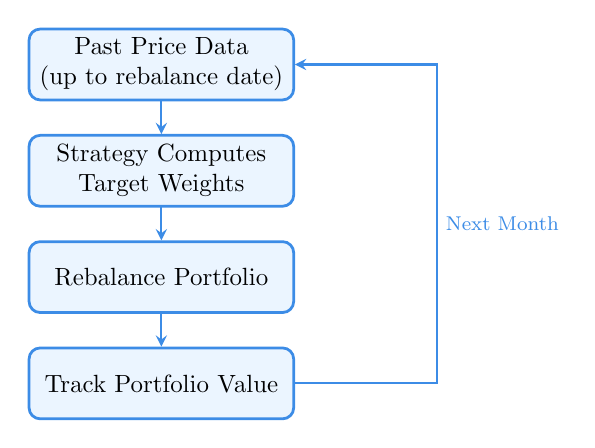
\begin{tikzpicture}[node distance=1.5cm, scale=0.9, every node/.style={scale=0.9}]
    \tikzstyle{block} = [rectangle, draw, fill=scrlightblue,
        text width=3.5cm, text centered, rounded corners=4pt, minimum height=1cm,
        line width=1pt, draw=scrblue]
    \tikzstyle{arrow} = [thick,->,>=stealth,color=scrblue]

    \node [block] (data) {Past Price Data\\(up to rebalance date)};
    \node [block, below of=data] (strategy) {Strategy Computes\\Target Weights};
    \node [block, below of=strategy] (rebalance) {Rebalance Portfolio};
    \node [block, below of=rebalance] (track) {Track Portfolio Value};

    \draw [arrow] (data) -- (strategy);
    \draw [arrow] (strategy) -- (rebalance);
    \draw [arrow] (rebalance) -- (track);
    \draw [arrow] (track.east) -- ++(2,0) |- node[near start, right, font=\footnotesize] {Next Month} (data.east);
\end{tikzpicture}
\end{center}

\vspace{0.3em}

\begin{alertblock}{Critical:}
Strictly rolling out-of-sample backtesting with no forward-looking information.
\end{alertblock}
\end{frame}

% Performance Metrics
\begin{frame}{What We're Measuring}
\begin{table}

\renewcommand{\arraystretch}{1.5}

\small
\begin{tabular}{l | l | r}
\toprule
\textbf{Metric} & \textbf{Definition} & \textbf{Focus} \\
\midrule
Total Return & Cumulative gain/loss (10 years) & Returns \\
CAGR & Annualised return & Returns \\
Volatility & Annualised standard deviation & Risk \\
Sharpe Ratio & Excess return per unit of risk & Risk Adjusted Performance \\
Max Drawdown & Largest peak-to-trough decline & Tail Risk\\
Sortino Ratio & Downside risk-adjusted return & Downside Risk\\
Turnover & Trading frequency (costs) & Implementation Risk \\
\bottomrule
\end{tabular}
\end{table}

\end{frame}

% Evaluation Criteria
\begin{frame}{Evaluation Framework}

\textbf{Performance}
\begin{itemize}
    \item Sharpe ratio, Sortino ratio, Maximum drawdown
\end{itemize}

\vspace{0.3cm}

\textbf{Regime Robustness}
\begin{itemize}
    \item Brexit (2016), COVID crash, 2022 equity-bond sell-off
\end{itemize}

\vspace{0.3cm}

\textbf{Implementation Feasibility}
\begin{itemize}
    \item Turnover, allocation stability, parameter sensitivity
\end{itemize}

\vspace{0.5cm}

\centering
\textit{Strategies are evaluated on performance, resilience, and implementability.}

\end{frame}



% Progress Update
\begin{frame}{Implementation Status}
\begin{columns}
\begin{column}{0.48\textwidth}
\textbf{Completed:}
\begin{itemize}
    \item Data pipeline (18 assets, 2015-2025)
    \item Backtesting engine
    \item Equal weight baseline
    \item Black-Litterman framework
\end{itemize}
\end{column}

\begin{column}{0.48\textwidth}
\textbf{→ In Progress:}
\begin{itemize}
    \item MVO implementation
    \item Black-Litterman views
    \item Risk Parity solver
    \item Performance analysis
\end{itemize}
\end{column}
\end{columns}

\vspace{1em}

\begin{block}{Coming Soon}
\begin{itemize}
    \item Full backtest results across all 4 strategies
    \item Regime analysis (bull/bear/crisis)
    \item Comprehensive research report
\end{itemize}
\end{block}
\end{frame}

% What This Research Means
\begin{frame}{Implications}
\begin{center}
\Large
\textcolor{scrdarkblue}{\textbf{Bridging the gap between theory and practice}}
\end{center}

\Large
\vspace{0.5cm}
\centering
Empirical test of whether a theoretical perfect portfolio survives real-world estimation errors and regime shifts 

\vspace{1cm}

\normalsize
\begin{center}
\textit{Academic finance says "here's the optimal solution"\\
We're asking: "does it actually work?"}
\end{center}

\end{frame}

% Follow Along
\begin{frame}{Want to Follow Along?}
\begin{center}
\Large
\textbf{GitHub Repository}\\
\vspace{0.5em}
\normalsize
\hyperlink{GitHub Link}{github.com/AP-Capital-Research/deep-dive-into-portfolio-optimisation}

\vspace{2em}

\Large
\textbf{Full Research Report}\\
\vspace{0.5em}
\normalsize
Expected publication: March 2026

\vspace{2em}

\textbf{Questions or feedback?}\\
Contact us at [rd01004@surrey.ac.uk]
\end{center}

\end{frame}

% Thank You
{
\watermark
\begin{frame}
\begin{center}
\Huge
\textcolor{scrdarkblue}{\textbf{Thank You}}

\vspace{2em}

\Large
We're excited to share our findings\\
with the quant finance community

\vspace{1em}

\normalsize
\textit{Stay tuned for the full results}
\end{center}

\end{frame}
}

\end{document}